\chapter{Decisiones operativas de marketing}

\section{Productos}

\subsection{Diseño de los productos}
Se muestran algunos objetivos en cuanto al diseño de este producto
\begin{itemize}
\item Se ofrecerá una alternativa diferente de enviar un paquete, usando los mismos medios de trasporte de nuestra ciudad.
\item Se brindara un servicio de calidad, seguro y confiable.
\item Fomentar la confianza en la tecnología, y la disminución de trafico en arequipa
\item Ayudar a personas que quieren trabajar y tienen un vehículo.
\end{itemize}
En cuanto a las características del producto se tiene lo siguiente:
\begin{itemize}
\item NOMBRE:    EASYCOURIER
\item LOGOTIPO: 
\includegraphics[width=0.2\textwidth]{easycourier}
\end{itemize}

\subsection{Plan de acción}
\begin{itemize}
\item Preparar el papeleo para la inscripción de la empresa en la sunarp con el nombre predispuesto anteriormente
\item Hacer llamadas a taxistas y personas que estén dispuestas a portar este logo, y acompañarnos en esta empresa.
\item Evaluar a cada transportista, para ver si esta apto para el puesto.
\item Implementar mecanismos de control y seguridad frente al envío de paquetes
\item Crear una pagina web y un aplicativo multiplataforma para cualquier consulta o servicio.
\end{itemize}

\section{Precios}

\subsection{Identificación de costos}
\label{sec:costos}
Identificamos los siguientes costos fijos:

\begin{itemize}
\item \textbf{S/. 256}: Servidores en la nube, Amazon EC2, máquinas del tipo t2.large (2 CPUs, 8GB RAM)
\item \textbf{S/. 600}: Alquiler de la oficina de desarrolladores
\item \textbf{S/. 150}: Recibos de luz y agua
\item \textbf{S/. 120}: Internet Claro de 8Mb
\item \textbf{5 x S/. 2000}: Salarios
\item \textbf{S/. 300}: Publicidad en redes sociales
\end{itemize}

No identificamos ningún costo variable.

\subsection{Política de precios}

Queremos brindar un servicio de calidad y fácil de usar. Pretendemos una penetración rápida y profunda en el mercado reduciendo el margen de ganancia al mínimo en un inicio, y luego incrementándolo una vez que los usuarios se acostumbren a la aplicación.

Tenemos dos frentes donde cobrar dinero. En primer lugar tenemos a los usuarios finales, a quienes se les ofrece un servicio de calidad por un precio razonable, no esperamos obtener ganancias de este grupo. De donde esperamos obtener ganancias es de cobrarle una comisión a los taxistas por cada encomienda que se les consiga. Durante los dos primeros meses que el taxista utilice la aplicación, gozará del 100\% de los beneficios de su trabajo, luego se le cobrará una comisión del 10\%. Esperamos que los taxistas ya familiarizados con la aplicación y conscientes de su beneficio, luego de dos meses de prueba gratis, estén dispuestos a pagar la comisión.


\section{Promoción}
\subsection{Publicidad}
De acuerdo a los objetivos de la publicidad se tienen los siguientes:
\begin{itemize}
\item Llegar al publico objetivo que se tenia en mente 
\item Que el publico conozca lo que ofrecemos en especial el valor agregado
\item Atraer a clientes potenciales como las empresas grandes, medianas o pequeñas.
\end{itemize}
Se cuenta con diversas estrategias de Promoción:
\begin{itemize}
\item Transmitir la facilidad de enviar un paquete a otro destino mediante las personas.
\item Dar a conocer nuestros servicios mediante vídeos, imágenes por las redes sociales
\item Hacer que el nombre de la empresa alcance un posicionamiento, mediante casos de éxito que se van ha ir dando en los primeros envíos.

\end{itemize}
\subsection{Fuerza de Ventas}
Para que el servicio sea muy consecuente se traza unos objetivos:
\begin{itemize}
\item Que mas del 80 por ciento de los conductores estén haciendo pedidos por día 
\item Que las personas reconozcan el nombre 
\item La reincidencia de pedir nuestros servicios por parte del cliente.
\end{itemize}
Teniendo en mente los objetivos a los cuales se quiere llegar se plantea lo siguiente:
\begin{itemize}
\item Promocionar el producto con descuentos el primer día, para que prueben el servicio, sin perder en cuenta los gastos previos a dicha promoción
\item Inundar las redes sociales, con el valor añadido de nuestros productos
\end{itemize}
\subsection{Relaciones Públicas}
Para que la empresa sea bien vista por nuestros clientes, se propone lo siguiente:
\begin{itemize}
\item Poner énfasis en la seguridad, que el cliente note el nivel de seguridad que se propone. 
\item Tener un control estricto con los conductores que entran 
\item Convencer a las empresas, que deben optar por nuestros servicios, así muchas mas empresas sabrán que existimos 
\end{itemize}
\section{Distribución}
\subsection{Definición de los canales de distribución}
Los objetivos planteados son:
\begin{itemize}
\item Lograr que el servicio este disponible las 24 horas del día. 
\item Impulsar la cantidad de peticiones, si se pone el servicio a manos de empresas pequeñas, tales como de comida, o de muebles.
\end{itemize}
Para lograr los objetivos propuestos de-acuerdo a los canales de distribución se tendrá que tomar en cuenta las siguientes estrategias:
\begin{itemize}
\item Pedidos a través del aplicativo o pagina web
\item Pedidos a través de celular 
\item Pedidos a través de las mismas oficinas 
\item Para que un conductor pueda entrar a la empresa, el tramite se hace directamente en oficinas.
\end{itemize}
\subsection{Plan de acción}
\begin{itemize}
\item Para soportar la cantidad de personas que harán peticiones al mismo tiempo, se necesita un servidor que soporte el 70 por ciento del rango objetivo.
\item Capacitar al personal que aceptara los conductores entrantes, para que sepa como evaluar al conductor.
\item Capacitar un numero de personas que vendan el servicio a las fabricas.
\end{itemize}
\section{Personas}
La atención al cliente es primordial, ya que debe cumplir los estándares de seguridad, planteados para eso el personal esta capacitado para saber atender una petición de servicio, o una oferta de afiliación, la capacitación cuenta con, saber tratar al cliente, saber tratar al conductor. 
Ademas se debe tener en cuenta que cada conductor deberá ser evaluado antes de hacerse parte de la empresa, cuyos requisitos son:
\begin{itemize}
\item SOAT
\item Revisión Técnica 
\item Si es taxi SETARE
\item Antecedentes policiales
\item Revisión Psicológica (Se hará dentro de la empresa)

\end{itemize}

\section{Evidencia Física}
La empresa contara con un local, donde se puedan recibir tanto clientes, como conductores, a los clientes se le dará un folleto el cual tendrá nuestros servicios, tarifas, y donde ubicarnos en las redes sociales.
A cada conductor autorizado se le dará un fotocheck, en donde estará el nombre de la empresa, el conductor y la placa del vehículo, también se le dará un sticker para que pegue en su auto.


\section{Procesos}

A continuación detallamos con diagramas de flujo los dos principales procesos de este proyecto. El primero es el registro de nuevos clientes y el segundo es el pedido de nuevas encomiendas; este último se expone desde los puntos de vista tanto del cliente como del taxista.

\begin{figure}[htb]
\centering
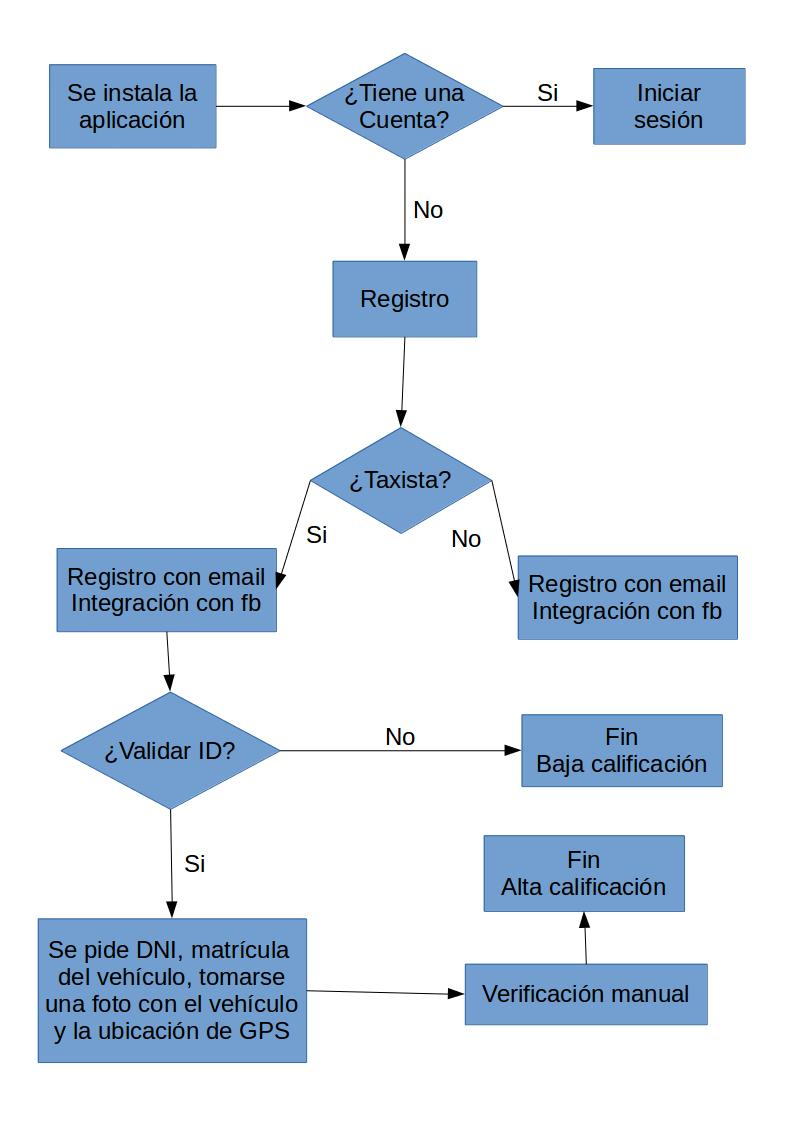
\includegraphics[width=0.8\textwidth]{./img/proceso_registro_nuevo_usuario.jpg}
\caption{Proceso de registro de un nuevo usuario} \label{fig:proc_nuevo_usuario}
\end{figure}

En la figura \ref{fig:proc_nuevo_usuario} vemos el proceso necesario para añadir un nuevo usuario al sistema, este puede ser un cliente o un taxista. En el caso de que sea un taxista, se pide un paso adicional: la verificación de identidad. Este paso es importante puesto que nos permite brindarle un servicio de calidad a los clientes, y tratamos de incentivarlo con un sistema de calificación, si te verificas obtienes una alta valoración, y si no lo haces tu valoración es muy baja, con lo que es menos probables que los usuarios te escojan a la hora de solicitar el servicio de courier. Pensamos realizar la verificación de forma manual, consultando la información del DNI y comparándola con la foto que nos envíe, lo mismo con el vehículo.


\begin{figure}[htb]
\centering
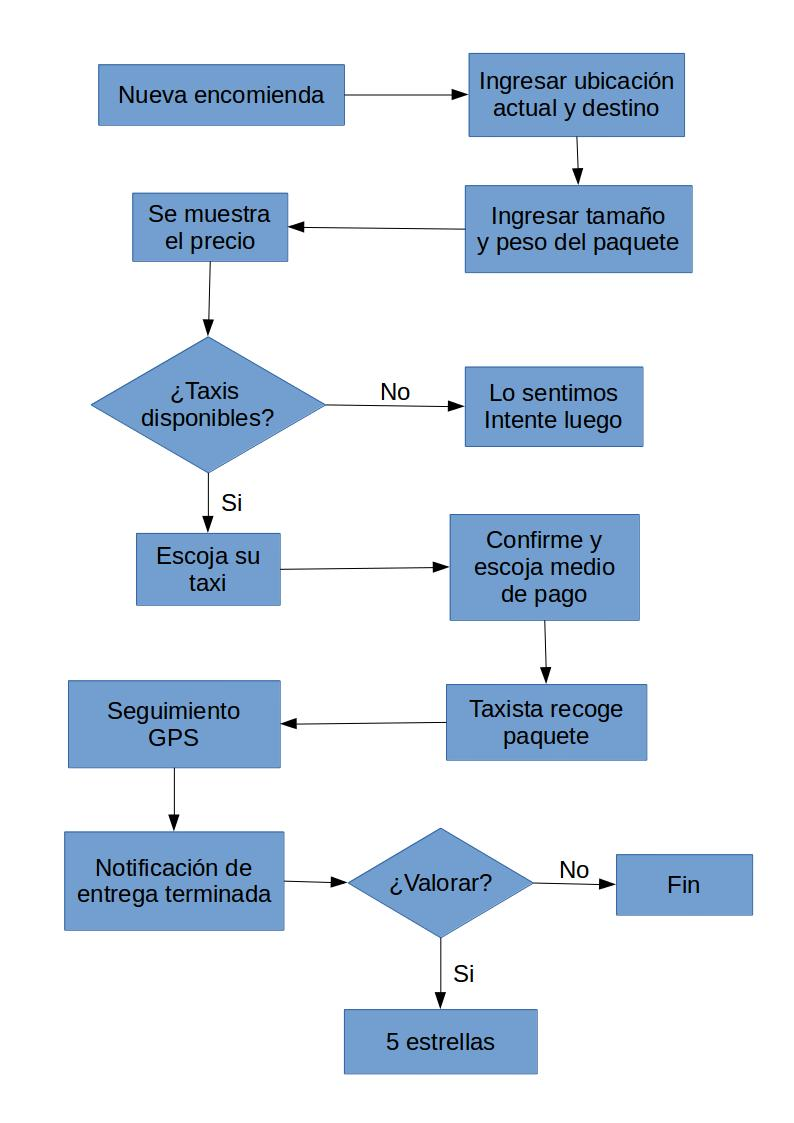
\includegraphics[width=0.8\textwidth]{./img/nueva_encomienda.jpg}
\caption{Proceso de solicitud de una nueva encomienda, desde el punto de vista del usuario final} \label{fig:proc_nueva_encomienda}
\end{figure}


\begin{figure}[htb]
\centering
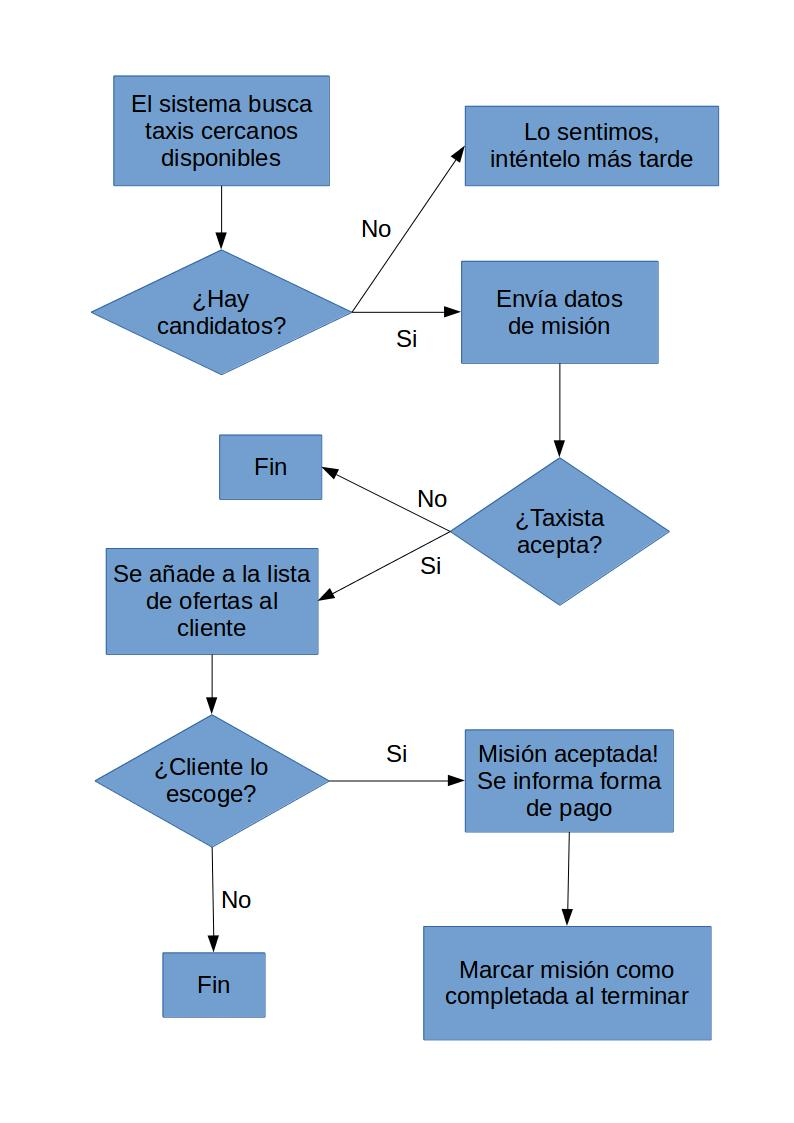
\includegraphics[width=0.8\textwidth]{./img/taxista.jpg}
\caption{Proceso de solicitud de una nueva encomienda, desde el punto de vista del taxista} \label{fig:proc_taxista}
\end{figure}


En la figuras \ref{fig:proc_nueva_encomienda} y \ref{fig:proc_taxista} se aprecia el proceso mediante el cual se solicita una nueva encomienda. El precio que se le muestra al cliente depende de la distancia del recorrido, así como del tamaño y peso del paquete. Este precio es calculado por nuestro sistema y no es negociable, de ese modo queremos crear una tarifa objetiva y estándar. Los usuarios finales obtienen una lista de taxistas que pueden cubrir el servicio, cada taxista con su respectiva valoración. Mientras el paquete se encuentra en el taxi, la aplicación hace un seguimiento GPS para que el cliente sepa donde se encuentra su paquete en todo momento. Una vez que el paquete llega a su destino, el cliente recibe una notificación y la opción para poder valorar el servicio del taxista. Puede llamar para ver si el paquete llego bien por ejemplo, y en base a eso calificar.

Los taxistas desde su punto de vista van recibiendo constantemente misiones de courier que pueden ir aceptando o ignorando. También es importante notar que al aceptar una misión, el taxista simplemente se añade a la lista de candidatos para el cliente, pero es en última instancia el cliente quien decide qué taxista realizará el servicio. Esta es otra forma de motivar que los taxistas tengan una buena calificación.